\chapter{Tipos de Gráficos} \label{app:chart}

Diferentes tipos de gráficos podem ser gerados depois das simulações. Alguns deles são:

\begin{figure}[htb!]
  \centering
  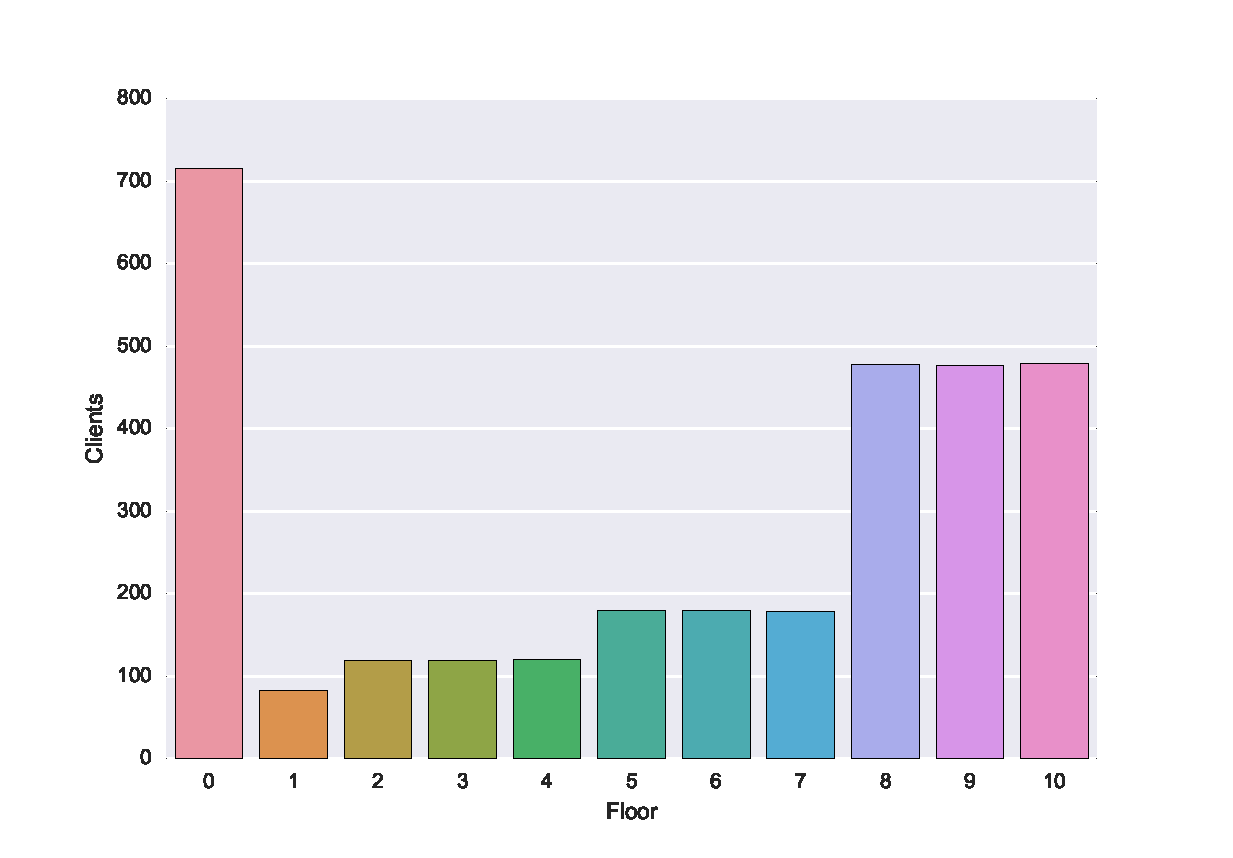
\includegraphics[scale=0.6]{img/results/Low-rise/5_Planning_Random/arrivalsPerFloor.eps}
  \caption{Chegadas por andar.}
  \label{fig:graphs:arrivalsperfloor}
\end{figure}

\begin{figure}[htb!]
  \centering
  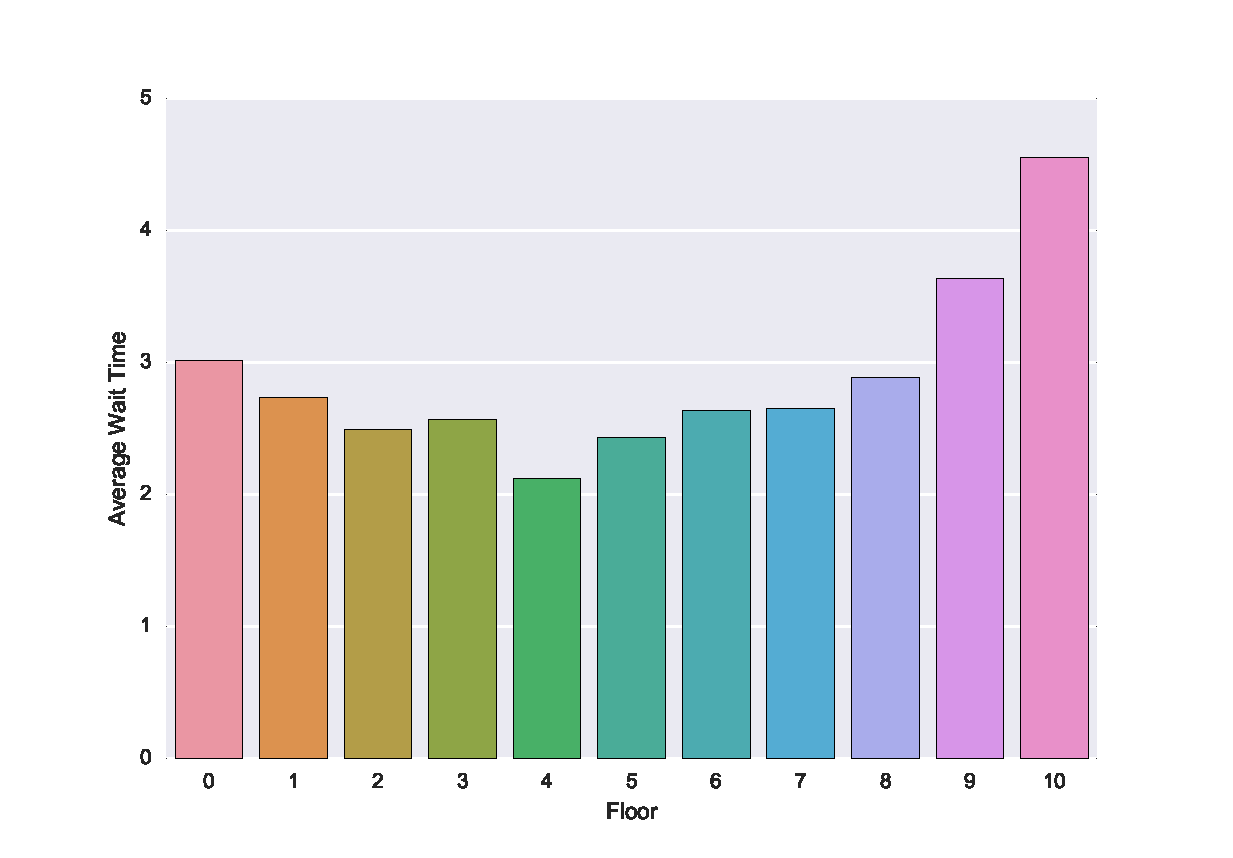
\includegraphics[scale=0.6]{img/results/Low-rise/5_Planning_Random/averageWaitTime.eps}
  \caption{Tempo médio de espera por andar.}
  \label{fig:graphs:averagewaittime}
\end{figure}

\begin{figure}[htb!]
  \centering
  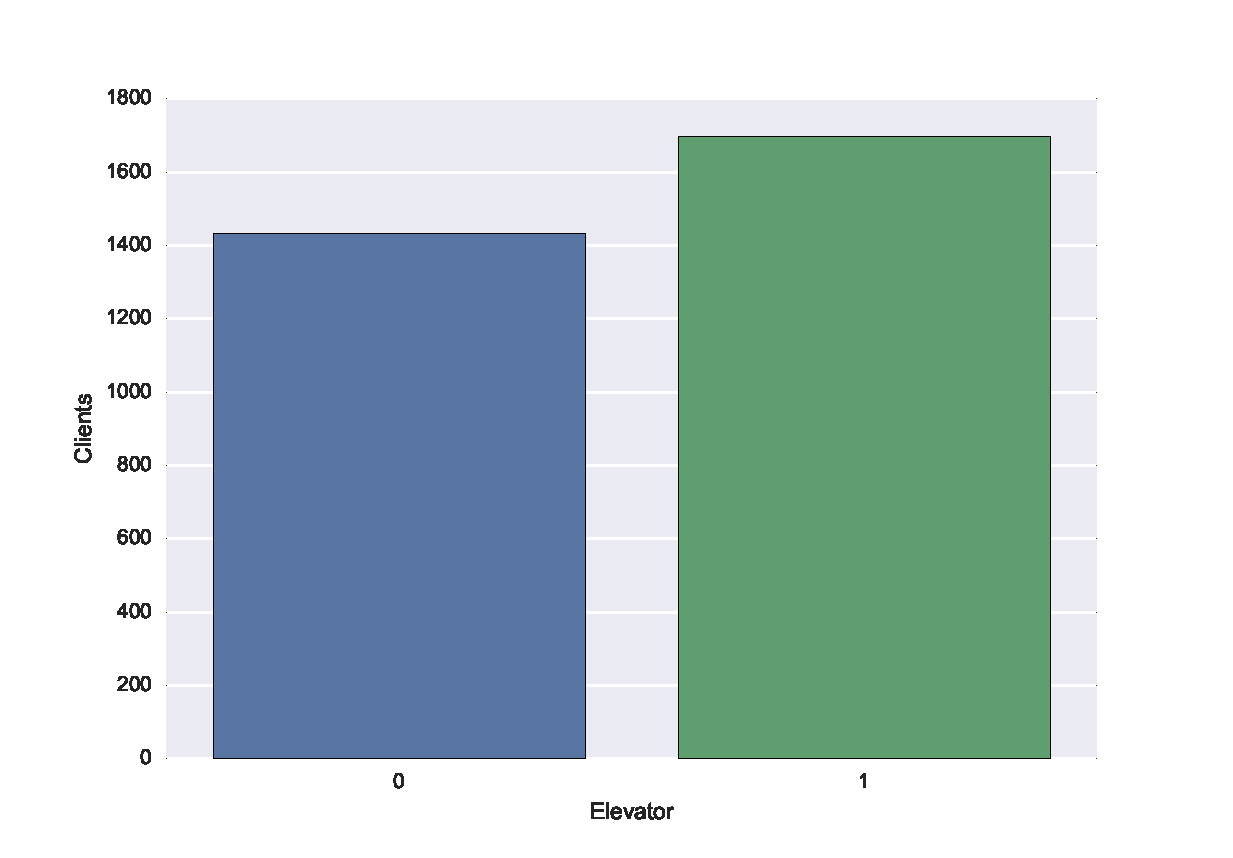
\includegraphics[scale=0.6]{img/results/Low-rise/5_Planning_Random/clientsPerElevator.eps}
  \caption{Clientes por elevador.}
  \label{fig:graphs:clientsperelevator}
\end{figure}

\begin{figure}[htb!]
  \centering
  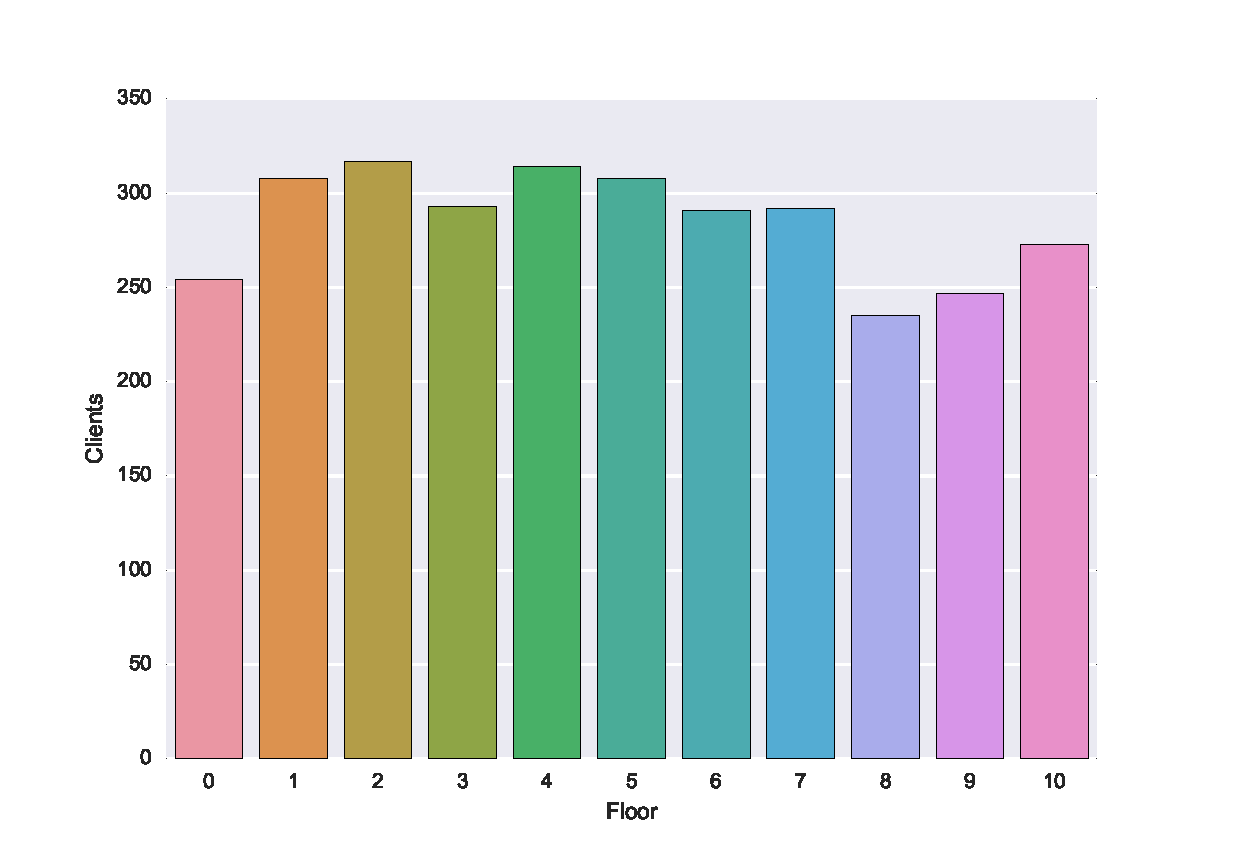
\includegraphics[scale=0.6]{img/results/Low-rise/5_Planning_Random/dropoffsPerFloor.eps}
  \caption{Total de clientes entregues por andar.}
  \label{fig:graphs:dropoffsPerFloor}
\end{figure}

\begin{figure}[htb!]
  \centering
  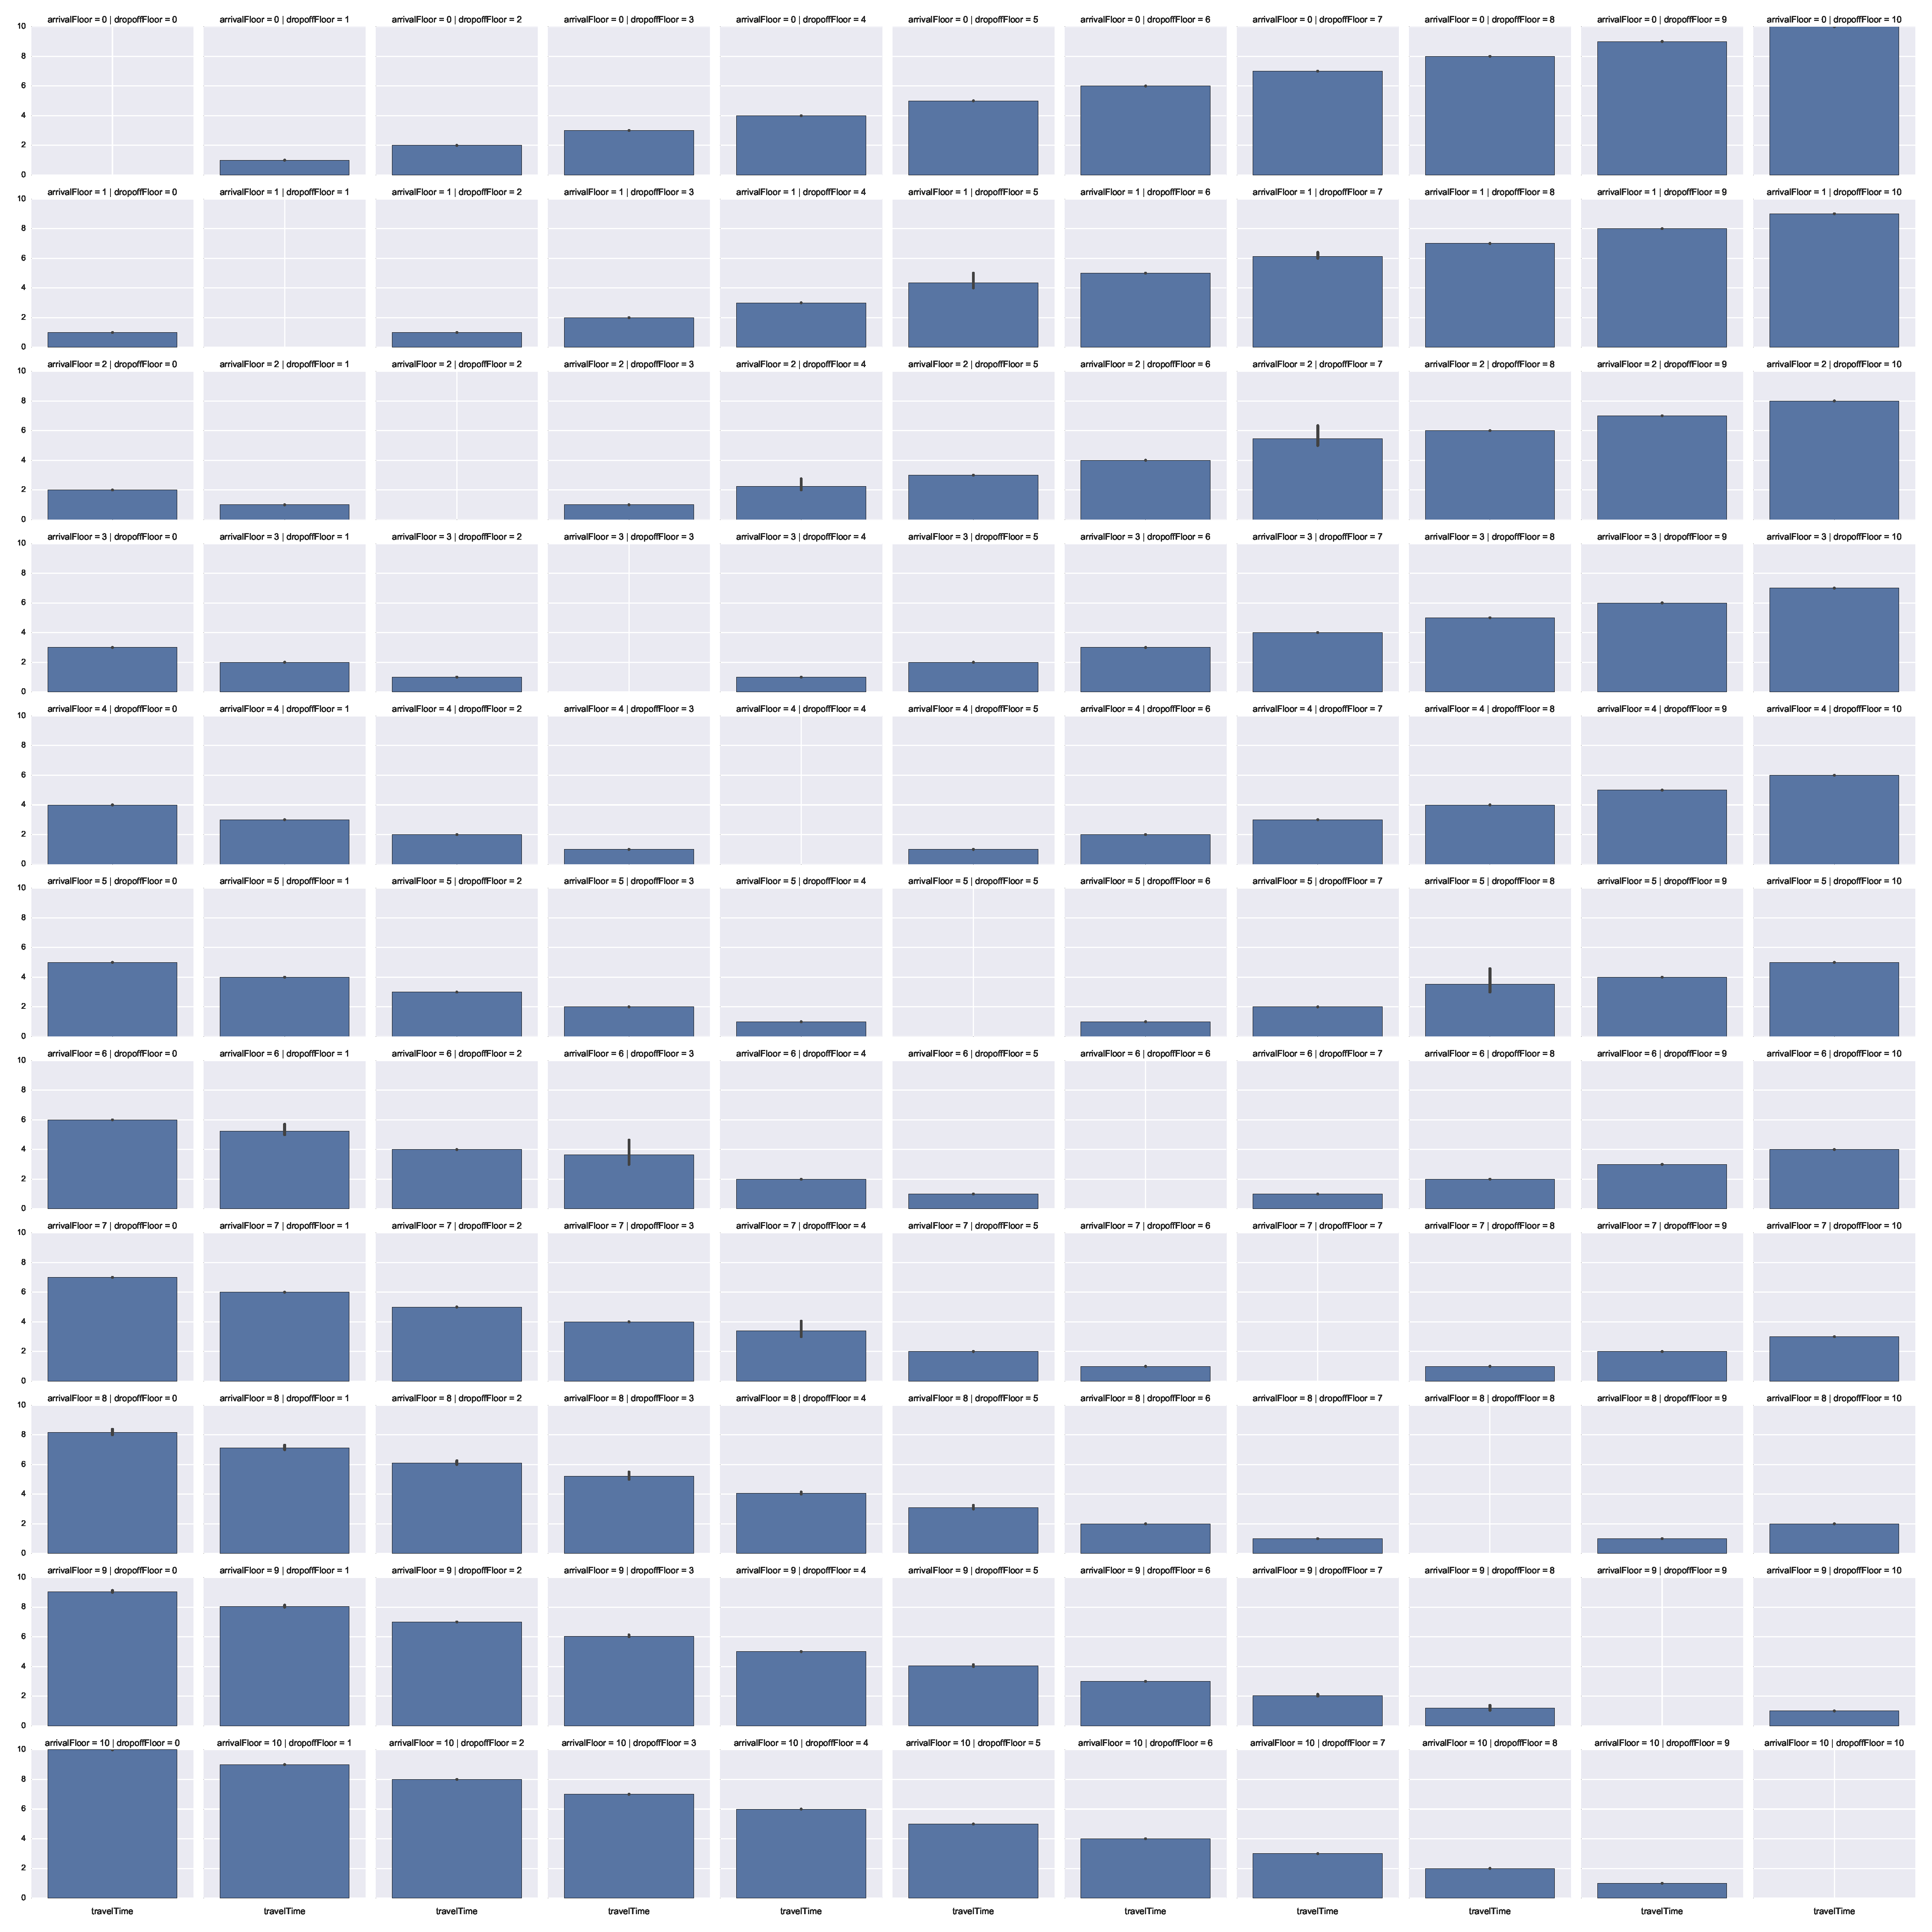
\includegraphics[scale=0.2]{img/results/Low-rise/5_Planning_Random/averageTravelTime.eps}
  \caption{Tempo médio de jornada de andar para andar.}
  \label{fig:graphs:averageTravelTime}
\end{figure}